%!TEX root = ../document.tex
\chapter{Repräsentation}
Die Strategie wird als neuronales Netz mit folgenden Eigenschaften dargestellt.
\begin{itemize}
\item Eingabeneuronen: 9
\item Hidden-Layer: 8
\item Neuronen je Hidden-Layer: 20;
\item Ausgabeneuronen: 6
\end{itemize}

Die Anzahl der Eingabeneuronen wird durch die 9 Eingabewerte bestimmt. Die 6 Ausgabeneuronen kommen durch die 5 aktiv beeinflussbaren Werte sowie durch die zusätzliche Option, Aufklärungspunkte für oder gegen Bevölkerung zu investieren, zustande.

Die Anzahl der Hidden-Layer und deren Neuronen wurde durch ständiges optimieren und testen ermittelt. Dabei erwiesen sich diese Anzahlen als optimal für das Problem. Mehr Hidden-Layer und Neuronen führten nur zu einer Laufzeitverlängerung und hatten keine Verbesserung der Güte zur Folge. Weniger Layer oder Neuronen pro Layer erwiesen sich im Gegensatz dazu als nicht geeignet, derart viele Parameter zu optimieren.

Ein Neuron wird innerhalb des Individuums wie in Abbildung \ref{fig:neuron} dargestellt.

\begin{figure}[tbph]
\centering
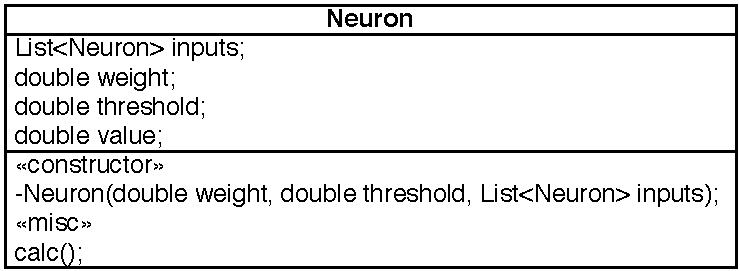
\includegraphics[width=0.5\linewidth]{pics/neuron}
\caption[Die Klasse Neuron]{Die Klasse Neuron}
\label{fig:neuron}
\end{figure}

Die Verknüpfung der Neuronen untereinander wird mit Hilfe des Konstruktors realisiert. Damit wird jedem Neuron eine Liste von eingehenden Neuronen übergeben. Dann wird die Methode \verb+calc()+ aufgerufen. Dort werden die Gewichte und Schwellwerte aufsummiert und mit Hilfe der Sigmoidfunktion der Wert des Neurons berechnet. Für alle Parameter außer \emph{Produktion} und der Option, Aufklärung für oder gegen die Bevölkerung zu investieren wird die Sigmoidfunktion wie in Formel \ref{equ:sig} verwendet. Für die beiden anderen Parameter wird eine Funktion benötigt, die Werte von $ -1 $ bis $ +1 $ liefert, um eine positive oder negative Investition darzustellen. Dafür wird der Tangens Hyperbolicus wie in Formel \ref{equ:tanh} verwendet.

\begin{equation}
\label{equ:sig}
sig(x) = \dfrac{1}{1+ e^{-x}}
\end{equation}

\begin{equation}
\label{equ:tanh}
\tanh(x) = \dfrac{1- e^{-2x}}{1+ e^{-2x}}
\end{equation}
